\part{研发用户指南}

\section{通用陆面模式中的自定义数据类型}

\subsection{格点数据}
CoLM中使用的地表覆盖类型、土壤属性、叶面积指数、流域划分、湖泊深度和树高等细分辨率数据,以及大气驱动和历史输出等粗分辨率数据都是格点数据。

为了处理高分辨率数据和进行并行计算,CoLM对所有格点数据进行分块。分块方案为:通过设置Namelist文件中的\texttt{DEF\_nx\_blocks}和\texttt{DEF\_ny\_blocks}两个变量的值,将经向180\textdegree W至180\textdegree E等分为\texttt{DEF\_nx\_blocks}段,将纬向90\textdegree N至90\textdegree S等分为\texttt{DEF\_ny\_blocks}段。对区域模拟,同样指的是对全球进行分块。格点数据分块进行读取和使用,以双精度浮点型数据为例,在代码(share/MOD\_DataType.F90)中“格点数据”的自定义数据类型为
\begin{lstlisting}[language=fortran, basicstyle=\linespread{1.0}\footnotesize\ttfamily, commentstyle=\color{olive}, numbers=left, numberstyle=\tiny, xleftmargin=1.5em,xrightmargin=0em, aboveskip=1em]
   type :: pointer_real8_2d
      real(r8), allocatable :: val (:,:)
   CONTAINS
      final :: pointer_real8_2d_free_mem
   END type pointer_real8_2d

   type :: block_data_real8_2d
      type(pointer_real8_2d), allocatable :: blk (:,:)
   CONTAINS
      final :: block_data_real8_2d_free_mem
   END type block_data_real8_2d
\end{lstlisting}
此外,代码中还定义了整型格点数据以及三维、四维格点数据。

格点数据建立在固定的经纬度网格上,经纬度网格在CoLM中使用自定义数据结构“网格”进行描述。网格数据结构包含了每个数据块的经纬度信息、全局位置、数据大小以及其他辅助信息。以下代码展示了如何在网格grid上建立双精度浮点型格点数据gdata2d,
\begin{lstlisting}[language=fortran, basicstyle=\linespread{1.0}\footnotesize\ttfamily, commentstyle=\color{olive}, numbers=left, numberstyle=\tiny, xleftmargin=1.5em,xrightmargin=0em, aboveskip=1em]
    type(grid_type),           intent(in)  :: grid
    type(block_data_real8_2d), intent(out) :: gdata2d

    ! 在网格grid上建立双精度浮点型格点数据gdata2d
    CALL allocate_block_data (grid, gdata2d)
\end{lstlisting}
模式中对格点数据类型定义了析构函数,因此,使用格点数据的代码结束时,无需编写释放内存的代码。

从netCDF文件中读取格点数据可使用以下函数(其中filename和dataname分别为文件名和文件中的变量名),
\begin{lstlisting}[language=fortran, basicstyle=\linespread{1.0}\footnotesize\ttfamily, commentstyle=\color{olive}, numbers=left, numberstyle=\tiny, xleftmargin=1.5em,xrightmargin=0em, aboveskip=1em]
   CALL ncio_read_block (filename, dataname, grid, gdata2d)
\end{lstlisting}

若netCDF文件中的数据包含时间维度,可使用以下函数(其中itime为文件中时间维度的值),
\begin{lstlisting}[language=fortran, basicstyle=\linespread{1.0}\footnotesize\ttfamily, commentstyle=\color{olive}, numbers=left, numberstyle=\tiny, xleftmargin=1.5em,xrightmargin=0em, aboveskip=1em]
   CALL ncio_read_block_time (filename, dataname, grid, itime, gdata2d)
\end{lstlisting}

以上函数allocate\_block\_data, ncio\_read\_block, ncio\_read\_block\_time对整型、浮点型以及二维、三维数据做了重载,因此,使用时函数名中未加数据类型及维数。

对格点数据的定位需要同时使用分块信息和网格信息,以下代码展示了如何对格点数据进行操作,
\begin{lstlisting}[language=fortran, basicstyle=\linespread{1.0}\footnotesize\ttfamily, commentstyle=\color{olive}, numbers=left, numberstyle=\tiny, xleftmargin=1.5em,xrightmargin=0em, aboveskip=1em]
    IF (p_is_io) THEN
        DO iblkme = 1, gblock%nblkme
            ib = gblock%xblkme(iblkme)
            jb = gblock%yblkme(iblkme)

            DO j = 1, grid%ycnt(jb)
                DO i = 1, grid%xcnt(ib)
                    ! 对gdata2d%blk(ib,jb)%val(i,j)进行操作
                ENDDO
            ENDDO
        ENDDO
    ENDIF
\end{lstlisting}
这段代码中,首先判断本进程是否为IO进程(格点数据仅位于读写进程的内存中,见第\ref{ch_parallel}节)。若是,则从gblock变量中循环获取分配给本进程的数据块的位置(代码中的ib和jb)。对分配给本进程的每个数据块,可进一步通过循环(代码中的j和i),对每个网格点上的数据进行操作。

\subsection{向量数据}

CoLM中的斑块(patch)、流域单元、非结构网格单元、水文响应单元、植被功能类型单元和植物群落单元等都具有不规则的形状,这些不规则形状单元在模式中使用细分辨率格点的集合进行表示。例如,使用0.5\textdegree 度经纬度网格单元进行陆面过程模拟时,在单元内部使用500米分辨率的地表覆盖类型数据建立次网格斑块单元,此时,一个斑块单元表示在一个0.5\textdegree 网格内部具有相同地表覆盖类型的500米细分辨率格点的集合。又如,使用流域单元进行陆面过程模拟时,根据90米高分辨率的水文学数据对模拟区域进行流域单元的划分,一个流域单元在模式中表示为90米细分辨率的格点的集合。

定义在不规则形状单元上的变量在模式中使用“向量”数据结构,为一维、二维或者三维数组,数组的最后一个维度的长度等于不规则单元的数量。例如定义在斑块上的叶面积指数
\begin{lstlisting}[language=fortran, basicstyle=\linespread{1.0}\footnotesize\ttfamily, commentstyle=\color{olive}, numbers=left, numberstyle=\tiny, xleftmargin=1.5em,xrightmargin=0em, aboveskip=1em]
    IF (p_is_worker) THEN
       allocate (lai (numpatch))
    ENDIF
\end{lstlisting}
这段代码中,首先判断本进程是否为worker进程(向量数据仅位于工作进程的内存中,见第\ref{ch_parallel}节)。若是,则定义一个一维数组存储叶面积指数的值,其长度等于分配到本进程的斑块的数量(numpatch)。

\subsection{格点数据和向量数据之间的映射}

陆面模式的输入数据(地表数据、大气驱动数据等)多为格点数据,而模式的基本单元为斑块等不规则单元,因此,需将格点数据映射到网格数据。CoLM中主要使用两种将格点数据映射到向量数据的方法,一种是面积加权平均,另一种是双线性插值。

以下代码定义和构建了由格点数据向斑块单元的面积加权平均映射,
\begin{lstlisting}[language=fortran, basicstyle=\linespread{1.0}\footnotesize\ttfamily, commentstyle=\color{olive}, numbers=left, numberstyle=\tiny, xleftmargin=1.5em,xrightmargin=0em, aboveskip=1em]
    type (grid_type) :: gforc
    type (pixelset_type) :: landpatch
    type (spatial_mapping_type) :: mg2p_forc

    ! 构建由定义在网格gforc上的格点数据向斑块单元的面积加权平均映射
    CALL mg2p_forc%build_arealweighted (gforc, landpatch)
\end{lstlisting}
具体实现时,面积加权平均方法先将格点数据映射到不规则单元内的细网格上,再对细网格进行加权平均,其可保证在映射的过程中变量是守恒的。上述映射只需在初始化时构建一次,调用以下函数进行使用
\begin{lstlisting}[language=fortran, basicstyle=\linespread{1.0}\footnotesize\ttfamily, commentstyle=\color{olive}, numbers=left, numberstyle=\tiny, xleftmargin=1.5em,xrightmargin=0em, aboveskip=1em]
    CALL mg2p_forc%grid2pset (forc_xy_t, forc_t)
\end{lstlisting}
其中,forc\_xy\_t为格点数据,forc\_t为向量数据。

以下代码定义和构建了由格点数据向斑块单元的双线性插值映射,
\begin{lstlisting}[language=fortran, basicstyle=\linespread{1.0}\footnotesize\ttfamily, commentstyle=\color{olive}, numbers=left, numberstyle=\tiny, xleftmargin=1.5em,xrightmargin=0em, aboveskip=1em]
    type (grid_type) :: gforc
    type (pixelset_type) :: landpatch
    type (spatial_mapping_type) :: mg2p_forc

    ! 构建由定义在网格gforc上的格点数据向斑块单元的双线性插值映射
    CALL mg2p_forc%build_bilinear (gforc, landpatch)
\end{lstlisting}
具体实现时,双线性映射方法将格点数据视为定义在经纬度网格点的中心位置,向量数据视为定义在不规则单元的重心位置,由包围不规则单元重心点的四个网格中心点向不规则单元进行插值。单独的双线性映射方法不能保证变量的守恒性,但与面积加权平均方法相比,使得插值后的变量在空间上较为平滑。上述映射同样只需在初始化时构建一次,调用以下函数进行使用
\begin{lstlisting}[language=fortran, basicstyle=\linespread{1.0}\footnotesize\ttfamily, commentstyle=\color{olive}, numbers=left, numberstyle=\tiny, xleftmargin=1.5em,xrightmargin=0em, aboveskip=1em]
    CALL mg2p_forc%grid2pset (forc_xy_t, forc_t)
\end{lstlisting}
其中,forc\_xy\_t为格点数据,forc\_t为向量数据。

模式结果通常以格点数据的方式输出,以增强可视化和结果分析的便利性,因此,需在输出时将定义在基本模拟单元上的向量数据映射到格点数据。向量数据向格点数据映射的构建与上述格点数据向向量数据映射的构建是相同的,使用时,以下函数
\begin{lstlisting}[language=fortran, basicstyle=\linespread{1.0}\footnotesize\ttfamily, commentstyle=\color{olive}, numbers=left, numberstyle=\tiny, xleftmargin=1.5em,xrightmargin=0em, aboveskip=1em]
    CALL mp2g_hist%pset2grid (hist_t, hist_xy_t, spv = filledvalue, msk = filter)
\end{lstlisting}
执行向量数据hist\_t向格点数据hist\_xy\_t的映射,其中spv和msk为两个可选参数。浮点数spv表示计算过程中不予考虑的填充值。msk为逻辑型向量数据,其第i个元素值为\texttt{TRUE}时表示此不规则单元参与映射,值为\texttt{FALSE}时表示不参与映射。例如,在输出湖泊温度时,可使用msk变量,将所有湖泊单元表示出来进行映射和输出。值得注意的是,当从向量数据向格点数据进行映射时,执行函数mp2g\_hist\%pset2grid得到的结果hist\_xy\_t表示格点内变量的总量,若要计算变量的均值,可先执行
\begin{lstlisting}[language=fortran, basicstyle=\linespread{1.0}\footnotesize\ttfamily, commentstyle=\color{olive}, numbers=left, numberstyle=\tiny, xleftmargin=1.5em,xrightmargin=0em, aboveskip=1em]
    CALL mp2g_hist%get_sumarea (sumarea, filter)
\end{lstlisting}
得到格点内参与映射的不规则单元的总面积sumarea,然后在每个格点内用变量的总量除以总面积得到均值。


\section{并行计算构架}\label{ch_parallel}

CoLM 2024版使用MPI(Massage Passing Interface)函数库实现在多核小型机、服务器以及超级计算机上的并行计算。

当使用多个进程运行模式时,所有进程被分为四类(见图~\ref{fig:fig_parallelization}),分别为主进程、读写进程、工作进程和回写进程。主进程(master)处理全局的输入输出和在运行过程中打印信息。读写进程(IO)进行数据的分发、收集和读写。工作进程(worker)执行模式过程。回写进程为可选项,专门用于历史文件的写出。一个工作组由一个读写进程和多个工作进程组成。

\begin{figure}[htpb]
    \centering
    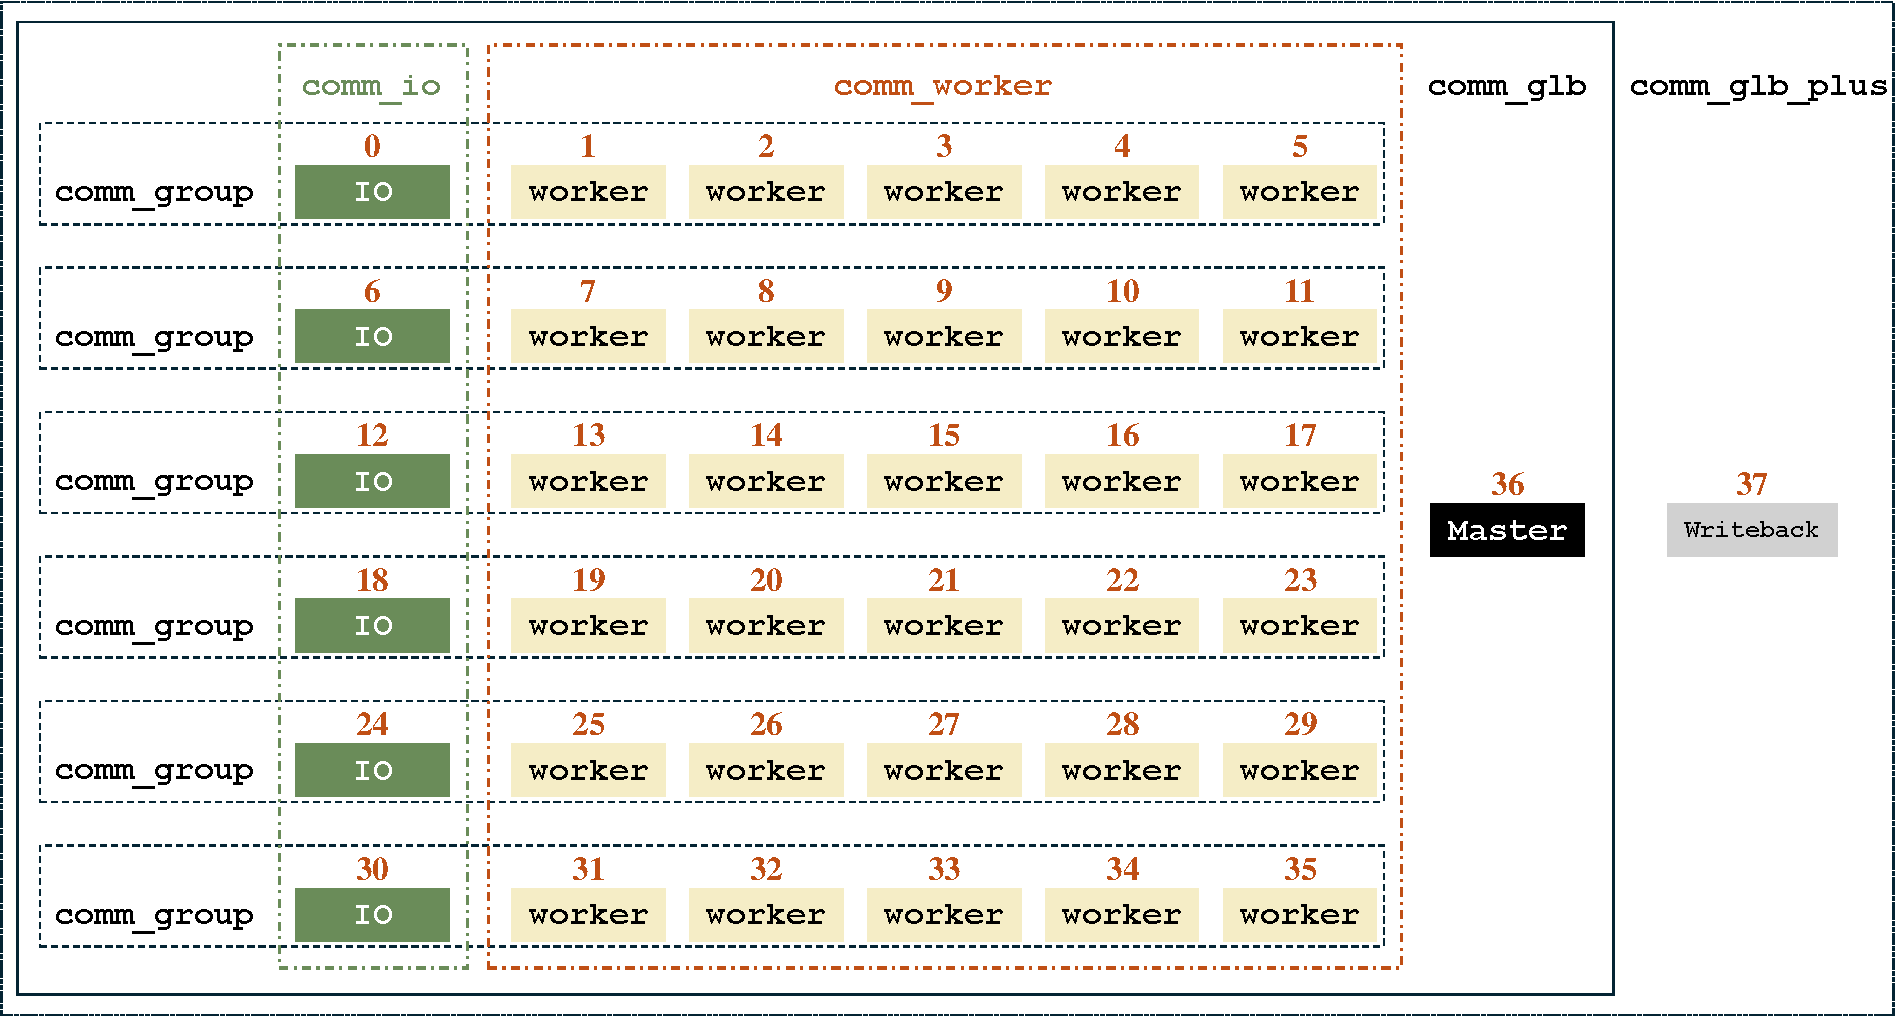
\includegraphics[width=\textwidth]{figures/并行计算图.pdf}
    \caption{CoLM 2024版并行计算构架示意图。其中所有进程被分为四类,分别为主进程、读写进程、工作进程和回写进程,数字标号0\textasciitilde 37为进程的全局编号。comm\_group为一个读写进程和多个工作进程组成的工作组通讯域,comm\_io为所有读写进程组成的通讯域,comm\_worker为所有工作进程组成的通讯域,comm\_glb为主进程、读写进程和工作进程组成的通讯域,comm\_glb\_plus为所有进程的通讯域。}
    \label{fig:fig_parallelization}
\end{figure}

并行运行模式时,模式以加权轮询的方式将数据块分配到工作组(见图~\ref{fig:fig_block}),每个工作组主要负责其分配到的数据块上的读写和模式计算。在工作组内,工作任务的分配以陆表单元(Element)为基本单位,每个陆表单元内部进一步划分的水文响应单元(HRU)、次网格单元(patch)、植被功能类型单元(PFT)以及植被群落单元(PC)等都分配到同一个进程上。工作组内任务的分配方法为将每个数据块上的陆表单元均匀分配,例如,某数据块有150个陆表单元,负责其计算的工作组有4个工作进程,将陆表单元按编号排序后,第1到4个工作进程分别进行第1到38、第39到76,第77到113,第114到150个陆表单元上的模拟。

\begin{figure}[htpb]
    \centering
    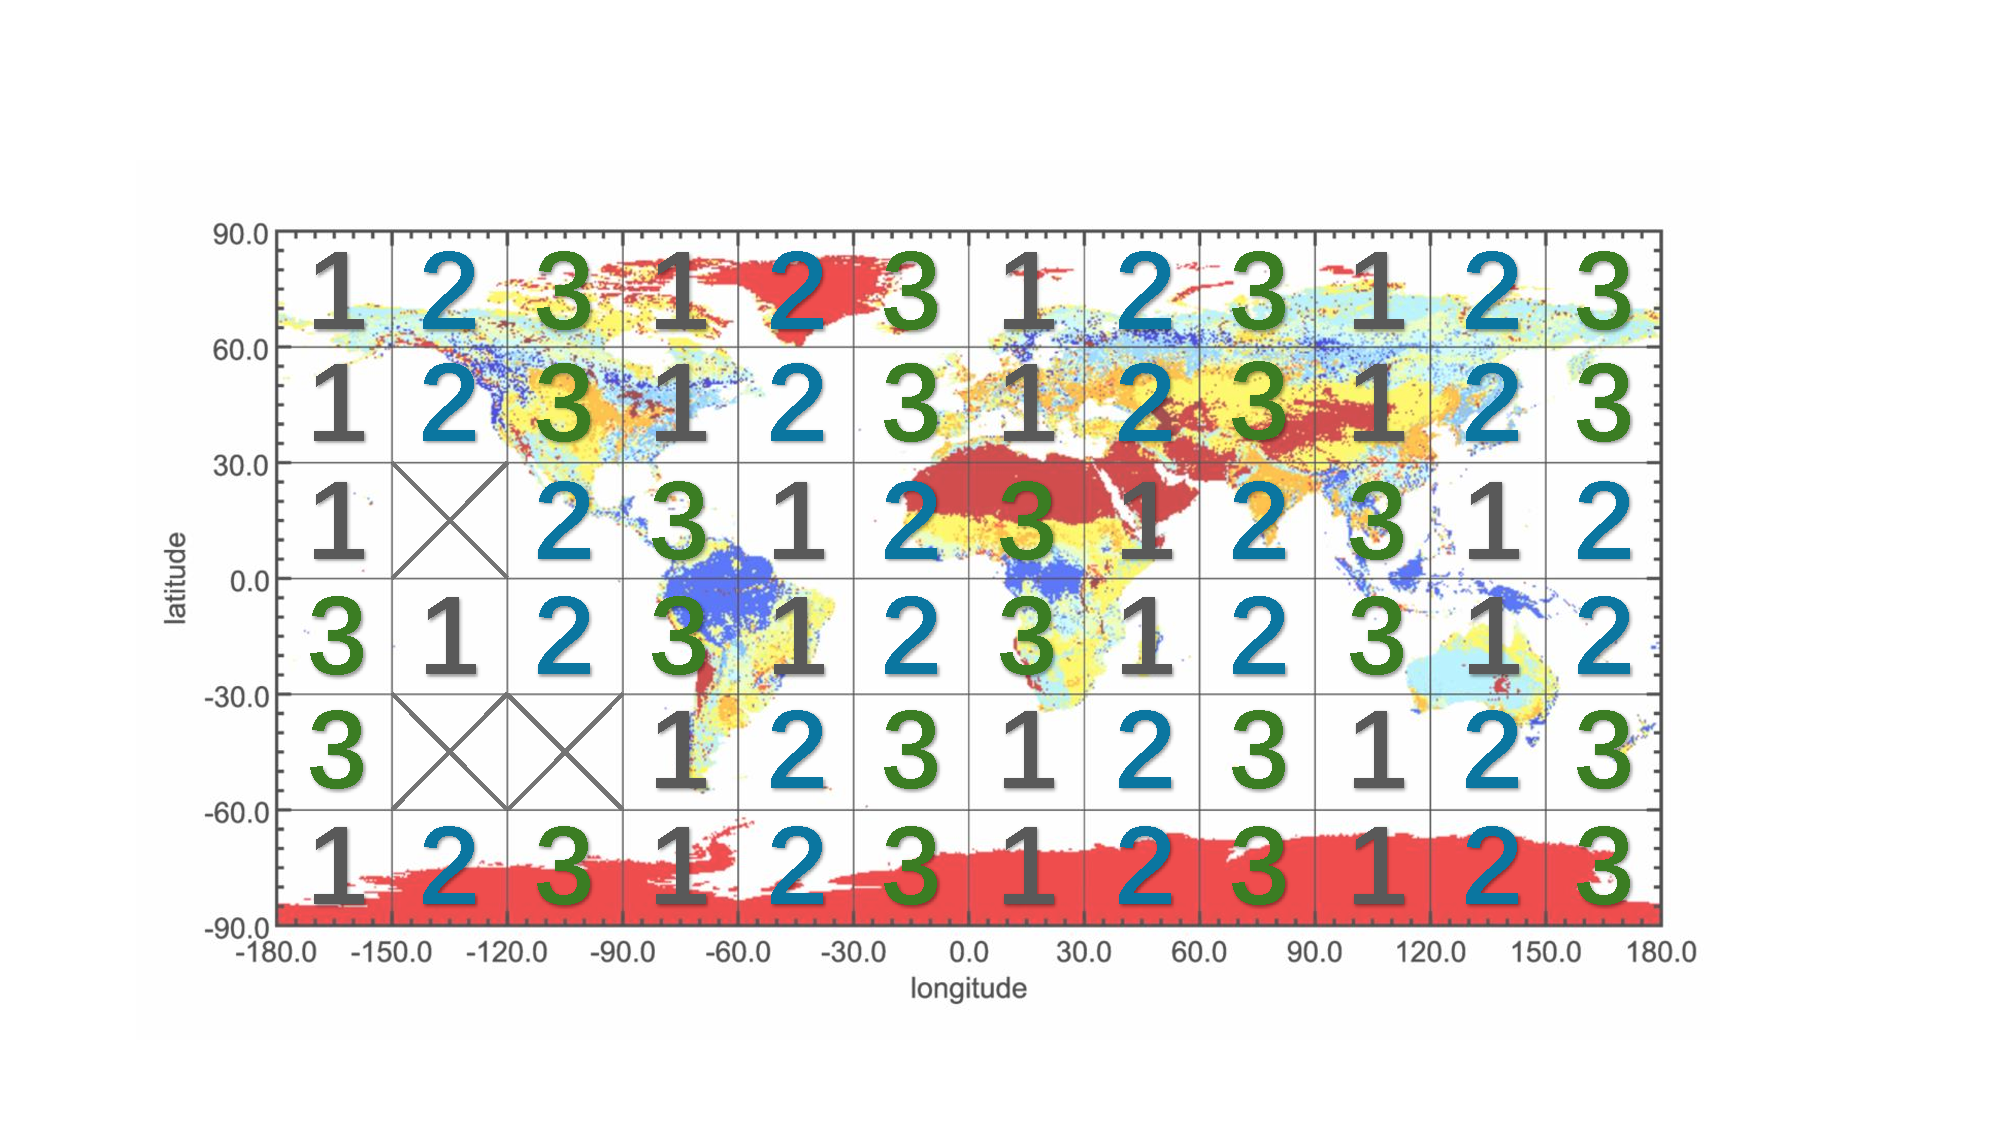
\includegraphics[width=\textwidth]{figures/数据分块示意图.pdf}
    \caption{CoLM 2024版数据分块及并行任务分配示意图。本例中将全球分为30\textdegree$\times$ 30\textdegree 的数据块。当使用3个工作组运行模式时,数据分块以轮询的方式分配到工作组,图中的数字1,2,3表示负责该数据块的工作组的编号。}
    \label{fig:fig_block}
\end{figure}

格点数据主要储存在读写进程(IO)的内存中,其读写有多种方式,可适应不同的计算环境。读入格点数据时,每个读写进程直接从外部文件中读入其负责的数据块上的数据。向外部文件写入格点数据有三种方式。第一种方式,当\texttt{DEF\_HIST\_mode}为'block'时,读写进程将每个数据块的内容写入单独的文件,这种方式通常具有最高的写文件速度,但分析结果时需要后处理程序拼接数据。第二种方式,当\texttt{DEF\_HIST\_mode}为'one'且\texttt{DEF\_HIST\_WriteBack}为\texttt{FALSE}时,由主进程在运行过程中从读写进程收集所有数据块的数据,进行拼接后将完整数据写出,这种方式不需要进行后期数据处理,但因收集数据时使用了阻塞通讯,在数据量较大时效率低、耗时长。第三种方式,当\texttt{DEF\_HIST\_mode}为'one'且\texttt{DEF\_HIST\_WriteBack}为\texttt{TRUE}时,模式将全局编号最大的进程独立出来作为回写进程,回写进程在运行过程中从读写进程收集所有数据块的数据,进行拼接后将完整数据写出,与第二种方式不同的是,读写进程向回写进程发送数据块上的数据时,使用的是非阻塞通讯,可不等待数据接收完成就继续向下运行。

向量数据主要储存在工作进程(worker)的内存中,其读写需通过读写进程(IO)。从外部文件读取向量数据时,读写进程首先读入其负责的数据块上的向量数据的子集,再分发给其工作组中的工作进程,分发过程通过进程之间的通讯实现。当向外部文件写入向量数据时,读写进程首先通过进程之间的通讯从其工作组中的工作进程收集数据,再按数据块将数据写入独立的文件。

因格点数据和向量数据分别位于读写进程和工作进程的内存中,格点数据和向量数据之间的映射均需通过进程之间的通讯实现。离线模拟时,大气驱动数据通常为格点数据,由读写进程读入后,按需发送至工作进程,再映射到向量数据。以经纬度网格进行历史数据输出时,需从工作进程发送以向量数据为形式的模拟结果至读写进程,再由读写进程累加到格点上。这些数据收发和累加映射的函数已封装在模块MOD\_SpatialMapping中,一般不需要开发者自己改写代码。

\section{代码的合作研发流程}

CoLM2024版本以及后续版本是开源代码,旨在建立开源共享和合作开发的“社区模型”发展策略。通过代码合作开发,充分了解用户在陆面生态方面的科学和技术需求。CoLM研发团队计划通过长期的年度培训,满足用户对CoLM模式开发和应用的技能需求。本节内容主要面向CoLM研发大团队和外部合作者,将详细介绍CoLM代码的规范研发流程和版本控制工具的规范使用。CoLM研发团队将邀请出色的新研发代码团队作为共同作者贡献CoLM新版本的技术手册。

\subsection{研发意向沟通}
外部合作者可以通过多种方式向CoLM研发团队详细概述模块开发计划,建立CoLM模块发展研发意向。CoLM学习班、CoLM研发论坛以及邮件沟通都可以与CoLM研发团队建立明确的研发意向。外部合作者通过沟通可以与CoLM研发团队互相了解各自的研发兴趣。若研发兴趣契合,外部合作者可以通过对模式研发计划的详细介绍,从CoLM研发团队获得具体的模式研发建议,包括代码修改建议、计算资源和人力资源建议等。外部研发者在完成资源准备和必要的培训之后,可以开始着手代码研发。

\subsection{模式研发的代码版本控制}
CoLM研发团队和外部合作者将统一使用github实现CoLM代码的版本控制。完成代码并测试后,研发者可以向CoLM主版本提交拉取请求(Pull Request)。研发者需要用github对代码进行远程仓库复刻、下载、修改和提交,并对远程仓库进行更新。

\subsubsection{用户的远程仓库复刻和代码的下载}
用户需要首先拥有自己的github账号(从github.com可申请),将CoLM的远程仓库(https://github.com/CoLM-SYSU/CoLM202X)复刻(点击fork)到自己账号下。仓库的复刻使得用户的新仓库保留了原仓库的所有提交历史、分支和文件,让用户既能参与开源贡献,又能进行独立实验,同时还保留了和原仓库的关联。

完成仓库复刻后,用户可以通过git clone命令克隆远程仓库到本地(在Linux系统下运行git clone):
\begin{lstlisting}[language=fortran, basicstyle=\linespread{1.0}\footnotesize\ttfamily, commentstyle=\color{olive}, numbers=left, numberstyle=\tiny, xleftmargin=1.5em,xrightmargin=0em, aboveskip=1em]
    git clone git@github.com:<账号名>/CoLM202X.git ./<本地仓库名>
\end{lstlisting}


或
\begin{lstlisting}[language=fortran, basicstyle=\linespread{1.0}\footnotesize\ttfamily, commentstyle=\color{olive}, numbers=left, numberstyle=\tiny, xleftmargin=1.5em,xrightmargin=0em, aboveskip=1em]
    git clone https://github.com/<账号名>/CoLM202X.git ./<本地仓库名>
\end{lstlisting}


推荐使用前者,但注意前者需要在机器上配置ssh,详细方法参见:

https://docs.github.com/en/authentication/connecting-to-github-with-ssh。

克隆完成后本地仓库拥有远程仓库现有的所有分支(branch),可以通过git checkout切换不同分支,便于多用户同时开发。

\subsubsection{代码的修改、提交和远程仓库更新}

用户在本地分支可以进行代码修改、调试和运行,github可以将任意文件的改动和原文件进行比较,实现代码修改的追踪:

\begin{lstlisting}[language=fortran, basicstyle=\linespread{1.0}\footnotesize\ttfamily, commentstyle=\color{olive}, numbers=left, numberstyle=\tiny, xleftmargin=1.5em,xrightmargin=0em, aboveskip=1em]
   git diff <文件名>
\end{lstlisting}



同时,用户可以查询本次修改包含哪些文件:

\begin{lstlisting}[language=fortran, basicstyle=\linespread{1.0}\footnotesize\ttfamily, commentstyle=\color{olive}, numbers=left, numberstyle=\tiny, xleftmargin=1.5em,xrightmargin=0em, aboveskip=1em]
   git status -uno
\end{lstlisting}

完成代码修改后,需确认代码修改:

\begin{lstlisting}[language=fortran, basicstyle=\linespread{1.0}\footnotesize\ttfamily, commentstyle=\color{olive}, numbers=left, numberstyle=\tiny, xleftmargin=1.5em,xrightmargin=0em, aboveskip=1em]
   git add <文件名>
\end{lstlisting}

确认完所有已修改代码后,需提交所有本次修改,并附上说明。

\begin{lstlisting}[language=fortran, basicstyle=\linespread{1.0}\footnotesize\ttfamily, commentstyle=\color{olive}, numbers=left, numberstyle=\tiny, xleftmargin=1.5em,xrightmargin=0em, aboveskip=1em]
   git commit -m “代码修改说明”
\end{lstlisting}

用户需要将所有修改上传远程仓库:

\begin{lstlisting}[language=fortran, basicstyle=\linespread{1.0}\footnotesize\ttfamily, commentstyle=\color{olive}, numbers=left, numberstyle=\tiny, xleftmargin=1.5em,xrightmargin=0em, aboveskip=1em]
   git push
\end{lstlisting}

若用户的远程仓库需要更新CoLM主版本的修改,可以点击github网页上用户页面的同步(Sync fork)按钮。

若本地仓库需要获取远程仓库同步过后的更新:

\begin{lstlisting}[language=fortran, basicstyle=\linespread{1.0}\footnotesize\ttfamily, commentstyle=\color{olive}, numbers=left, numberstyle=\tiny, xleftmargin=1.5em,xrightmargin=0em, aboveskip=1em]
   git pull
\end{lstlisting}


若有代码冲突需要手动解决冲突,并确认修改。

详细的github操作解说,请查阅github官方文档:

英文:https://docs.github.com/en

中文:https://docs.github.com/zh


\subsubsection{代码的测试}

研发者初步完成代码开发后,在申请CoLM主版本合并前,需要用测试软件包完成代码的测试。若测试存在失败项目,需要修改代码后,重新测试直到所有测试通过。测试软件包含有22个测试项目,见表~\ref{测试列表}涉及多驱动场、多模块和多分辨率的不同组合。新研发代码需要兼容所有待测试的配置组合,所有测试目前仅限于冒烟测试,即保证模式完成一年的运行,无编译报错、运行出错、nan值或各种平衡检查报错。

\begin{table}[!htbp]
\renewcommand{\arraystretch}{1.5}
\centering
\caption{测试案例配置列表}\label{测试列表}
\begin{tabular}{
ccccccc} \toprule
\textbf{序号} & \textbf{分辨率} & \textbf{次网格} & \textbf{土壤模型} & \textbf{BGC} & \textbf{作物} & \textbf{驱动} \\ \midrule
1 & 2.5$\times$1.875 & PC & VG & 开 & 关 & CRUJRA \\
2 & 2.5$\times$1.875 & PFT & VG & 开 & 关 & CRUJRA \\
3 & 2.5$\times$1.875 & PC & VG & 开 & 开 & CRUJRA \\
4 & 2.5$\times$1.875 & PFT & VG & 开 & 开 & CRUJRA \\
5 & 2.5$\times$1.875 & PC & VG & 关 & 关 & CRUJRA \\
6 & 2.5$\times$1.875 & PFT & VG & 关 & 关 & CRUJRA \\
7 & 2.5$\times$1.875 & IGBP & VG & 关 & 关 & CRUJRA \\
8 & 2.5$\times$1.875 & USGS & VG & 关 & 关 & CRUJRA \\
9 & 2.5$\times$1.875 & PC & CB & 开 & 关 & CRUJRA \\
10 & 2.5$\times$1.875 & PFT & CB & 开 & 关 & CRUJRA \\
11 & 2.5$\times$1.875 & PC & CB & 开 & 开 & CRUJRA \\
12 & 2.5$\times$1.875 & PFT & CB & 开 & 开 & CRUJRA \\
13 & 2.5$\times$1.875 & PC & CB & 关 & 关 & CRUJRA \\
14 & 2.5$\times$1.875 & PFT & CB & 关 & 关 & CRUJRA \\
15 & 2.5$\times$1.875 & IGBP & CB & 关 & 关 & CRUJRA \\
16 & 2.5$\times$1.875 & USGS & CB & 关 & 关 & CRUJRA \\
17 & 0.1$\times$0.1 & PC & VG & 开 & 关 & CRUJRA \\
18 & 0.1$\times$0.1 & PC & VG & 关 & 关 & CRUJRA \\
19 & 0.1$\times$0.1 & PC & VG & 开 & 关 & ERA5 \\
20 & 0.1$\times$0.1 & PC & VG & 关 & 关 & ERA5 \\
21 & 0.1$\times$0.1 & PC & VG & 开 & 关 & ERA5LAND \\
22 & 0.1$\times$0.1 & PC & VG & 关 & 关 & ERA5LAND \\
\bottomrule
\end{tabular}
\end{table}


在运行测试软件包之前,需要根据特定系统及数据地址,配置machine.config和batch.config,详细介绍参见~\ref{辅助工具包}。测试软件包由create\_test、TestLists和SummaryTest.bash三个主要脚本组成,create\_test的创建模式根据TestLists中的测试项目设置,在研发者指定的路径下创建22个测试案例,运行案例并检查结果,SummaryTest将所有案例的检查结果进行汇总并打印。测试案例的创建需要用到create\_newcase脚本。完成测试案例创建后,create\_test将检查案例是否创建成功,并同时编译22个测试案例。create\_test脚本在run/scriopts目录下,其详细语法如下:

\begin{lstlisting}[language=fortran, basicstyle=\linespread{1.0}\footnotesize\ttfamily, commentstyle=\color{olive}, numbers=left, numberstyle=\tiny, xleftmargin=1.5em,xrightmargin=0em, aboveskip=1em]
   ./create_test -n {测试工作路径} [-f {测试列表}][-m {运行方式}][-t {测试类型} [-r {重启时间}]]
\end{lstlisting}

研发者需要指定{测试工作路径},用于存储测试案例的运行结果、配置、代码以及附属生成的地表数据、重启数据以及测试状态文件TestStatus。{测试列表}和{运行方式}为脚本可选参数。{测试列表}参数缺省时,将使用默认测试列表文件run/scripots/TestLists,包含22个已定义测试案例。研发者可以根据修改TestLists文件自定义测试列表。研发者可以通过{运行方式}设置create\_test的运行方式,可选{运行方式}包括以下4种:

a) Create: 根据<测试列表>创建并编译所有测试案例。

b) CreateNoMkSrf:根据<测试列表>创建所有案例,同时根据分辨率链接现有地表数据(landdata)

c) Run:运行已创建的测试案例,并检查运行结果。运行包括地表数据制作(mksrfdata.x的运行)、初始化(mkinidata.x的运行)和模式正式运行(colm.x的运行)

d) RunNoMkSrf:运行已创建的测试案例,并检查运行结果。但运行不包括地表数据制作(mksrfdata.x的运行),仅包括初始化(mkinidata.x的运行)和模式正式运行(colm.x的运行)

完整测试通常需要两步,1)创建测试案例和2)运行测试案例。根据研发代码的具体内容,研发者可以选择两种不同的测试方式。若研发内容不影响地表数据的制作,研发者可以选择免地表数据制作测试:

\begin{lstlisting}[language=fortran, basicstyle=\linespread{1.0}\footnotesize\ttfamily, commentstyle=\color{olive}, numbers=left, numberstyle=\tiny, xleftmargin=1.5em,xrightmargin=0em, aboveskip=1em]
   ./create_test -n {测试工作路径} -m CreateNoMkSrf
   ./create_test -n {测试工作路径} -m RunNoMkSrf
\end{lstlisting}

若研发内容影响地表数据制作,研发者须选择完整测试:

\begin{lstlisting}[language=fortran, basicstyle=\linespread{1.0}\footnotesize\ttfamily, commentstyle=\color{olive}, numbers=left, numberstyle=\tiny, xleftmargin=1.5em,xrightmargin=0em, aboveskip=1em]
   ./create_test -n {测试工作路径} -m Create
   ./create_test -n {测试工作路径} -m Run
\end{lstlisting}

所有测试案例在运行结束后,都会自动运行check\_mksrf.submit、check\_init.submit和check\_case.submit检测运行结果,并将检查结果存放测试状态文件TestStatus中。每个测试案例均有专属的测试状态文件TestStatus,TestStatus存放在测试案例的工作目录中。TestStatus可能包含以下七项内容:

1) CreateCase: 案例创建

2) compile: 编译

3) Submit\_Mksrfdata: 运行地表制作程序

4) Submit\_Mkinidata: 运行初始化程序

5) Submit\_Case: 运行主程序

6) Submit\_Restart: 如果是重启测试,还将包括运行重启程序的项目

7) RestartMatch: 如果是重启测试,还将包括重启结果比较项目

以上每一项均可能存在三种测试状态:

a)PEND 延迟状态,代表该项内容正在进行或尚未检测

b)FAIL 失败状态,代表该项内容经过检测后已经失败

c)PASS 通过状态,代表该项内容已经成功的通过检测

{测试类型}包括冒烟测试(SMS)和重启测试(RES)两类,该选项缺省为冒烟测试:

a) SMS:冒烟测试,按预设配置运行模型一年(2005.1.1-2005.12.31),检测运行结果是否顺利结束,是否包含nan,是否通过各类平衡测试。

b) RES:重启测试,按预设配置按两种方式运行模型,第一种完整运行模型4天(默认:2004.12.30-2005.1.2),第二种方式,基于第一种方式的重启文件从第三天开始(默认:2005.1.1)继续运行模型2天。重启测试除冒烟测试的检测外,同时比较两种方式后两日的模拟结果是否一致。

若测试类型为重启测试,可以通过-r选项设置重启时间,重启时间缺省为2005年1月1日。

例:

1. 运行免地表数据制作的重启测试,重启时间点为2005年1月1日
\begin{lstlisting}[language=fortran, basicstyle=\linespread{1.0}\footnotesize\ttfamily, commentstyle=\color{olive}, numbers=left, numberstyle=\tiny, xleftmargin=1.5em,xrightmargin=0em, aboveskip=1em]
   ./create_test -n {测试工作路径} -m RunNoMkSrf -t RES
\end{lstlisting}

2. 创建免地表数据制作的重启测试,重启时间点为2005年2月1日
\begin{lstlisting}[language=fortran, basicstyle=\linespread{1.0}\footnotesize\ttfamily, commentstyle=\color{olive}, numbers=left, numberstyle=\tiny, xleftmargin=1.5em,xrightmargin=0em, aboveskip=1em]
   ./create_test -n {测试工作路径} -m CreateNoMkSrf -t RES -r 2005-02-01
\end{lstlisting}


完成测试后,通过运行汇总脚本SummaryTest.bash可以将每个案例测试状态的每一项内容进行有汇总打印。除此之外,SummaryTest.bash还将检测每个案例的运行中是否存在水分、能量和碳平衡问题,以及检测变量中是否存在nan值。SummaryTest.bash在run/scripts目录下,其语法如下:

\begin{lstlisting}[language=fortran, basicstyle=\linespread{1.0}\footnotesize\ttfamily, commentstyle=\color{olive}, numbers=left, numberstyle=\tiny, xleftmargin=1.5em,xrightmargin=0em, aboveskip=1em]
   ./SummaryTest.bash -n {测试工作路径} [-f {测试列表}][-i {测试项目}][-t {测试类型}]
\end{lstlisting}

<测试工作路径>和<测试列表>是研发者create\_test时指定的测试案例的工作路径和测试列表。<测试列表>参数缺省时,将使用默认测试列表文件run/scripots/TestLists。<测试项目>除测试状态文件TestStatus中的七项内容之外,还可选择‘All’打印所有测试案例的所有项目;若为TestStatus七项之一,则打印所有案例的其中一项。<测试类型>包括冒烟测试(SMS)和重启测试(RES)两类,此处设置须与创建和运行测试设置的测试类型一致:

例:

1. 打印汇总所有测试案例所有项目的冒烟测试结果:

\begin{lstlisting}[language=fortran, basicstyle=\linespread{1.0}\footnotesize\ttfamily, commentstyle=\color{olive}, numbers=left, numberstyle=\tiny, xleftmargin=1.5em,xrightmargin=0em, aboveskip=1em]
   ./SummaryTest.bash -n {测试工作路径} -i 'All'
\end{lstlisting}

2. 打印汇总所有测试项目中和正式运行结果相关的冒烟测试结果:

\begin{lstlisting}[language=fortran, basicstyle=\linespread{1.0}\footnotesize\ttfamily, commentstyle=\color{olive}, numbers=left, numberstyle=\tiny, xleftmargin=1.5em,xrightmargin=0em, aboveskip=1em]
   ./SummaryTest.bash -n {测试工作路径} -i 'Submit_Case'
\end{lstlisting}

3. 打印汇总所有测试案例所有项目的重启测试结果:

\begin{lstlisting}[language=fortran, basicstyle=\linespread{1.0}\footnotesize\ttfamily, commentstyle=\color{olive}, numbers=left, numberstyle=\tiny, xleftmargin=1.5em,xrightmargin=0em, aboveskip=1em]
   ./SummaryTest.bash -n {测试工作路径} -t RES
\end{lstlisting}


\subsubsection{代码的拉取请求(Pull Request)}

完成代码测试后,研发者寻求将CoLM新代码融入CoLM主版本代码中,需要进行拉取请求,拉取请求按钮在github研发者CoLM分支主页上。并联系CoLM研发团队,并进行代码功能演示。CoLM研发团队根据代码完善程度,赋予拉取请求不同状态:

a)工作状态:研发代码功能并未完整,尚需进一步改善;

b)等候状态:CoLM研发团队并未准备好将新代码融入CoLM主版本;

c)就绪状态:CoLM研发团队已准备好将新代码融入CoLM主版本,但还需最终测试。

在代码完成最终测试,CoLM研发团队完成最终代码审查,新代码将进入CoLM主版本。
% \section{网格的定义}
